\documentclass[french]{beamer}

\usepackage[utf8]{inputenc}
\usepackage[T1]{fontenc}
\usepackage{lmodern}
\usepackage{babel}
\usepackage{tikz}
\usetikzlibrary{arrows}

\usetheme{PaloAlto}

\tikzset{
  treenode/.style = {align=center, inner sep=0pt, text centered,
    font=\sffamily},
  arn_equi/.style = {treenode, circle, white, draw=green, fill=green, text width=1em},
  arn_notequi/.style = {treenode, circle, white, draw=red,fill=red, text width=1em},
  arn_new/.style = {treenode, circle, white, draw=blue,fill=blue, text width=1em},
  arn_null/.style = {treenode, rectangle, draw=black,minimum width=0.5em, minimum height=0.5em}
}


%Pour le TITLEPAGE
\title{CPROJ}
\subtitle{Rapport du Projet}
\author[]{MARINO Isabelle 21306227,\\ TIRACHINE Hafça 21307587,\\JACQUETTE Pierrick 21305551}
\date{Avril 2016}
\institute[L3 S6-- Informatique]{Université Paris 7 Diderot}


\begin{document}

\begin{frame}
	\titlepage
\end{frame}

\section{AVL}
\begin{frame}{Stockage des Ways et des Nodes}
	\textbf{AVL} : C'est un ABR (arbre binaire de recherche) équilibré.
	On n'a pas besoin de conserver un ordre.
	\visible<2-3>{	
		Les opérations dont on a besoin (n est le nombre d'élément):
	}
	\begin{itemize}
	\item<2-3> \textbf{Insertion} : $\theta$(log n) : la hauteur de l'arbre
	\item<3-> \textbf{Recherche} : $\theta$(log n) : la hauteur de l'arbre
\end{itemize}
\end{frame}

\begin{frame}{Equilibrage lors d'une insertion}
\framesubtitle{Rotation simple gauche et droite}
	\begin{tabular}{ccc}
		 \multicolumn{2}{l}{
		 	\visible<1-4>{
	 			Diff de profondeur des ss-arbre de 2 et le FD une diff de 1.
	 		}
		 }
		 \\
	 	\visible<1-4>{		
			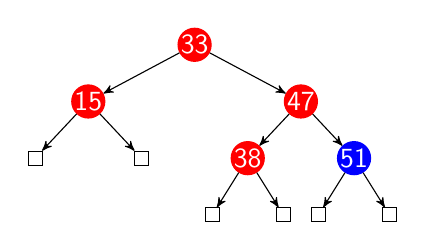
\begin{tikzpicture}[->,>=stealth',level/.style={sibling distance = 2.7cm/#1,level distance = 0.72cm}]
				\node [arn_notequi] {33}
		 				child{ node [arn_notequi] {15} 
		        			child{ node [arn_null] {}
						}
						child{ node [arn_null] {}
						}
		            	}                            
		    		    child{ node [arn_notequi] {47}
		            		child{ node [arn_notequi] {38} 
		            		    child{ node [arn_null] {}
							}
							child{ node [arn_null] {}
							}
		            		}
		            		child{ node [arn_new] {51}
		            		    child{ node [arn_null] {}
							}
							child{ node [arn_null] {}
							}
		            		}
					}
			; 
			\end{tikzpicture}
		}
		&
		\visible<2-4>{
			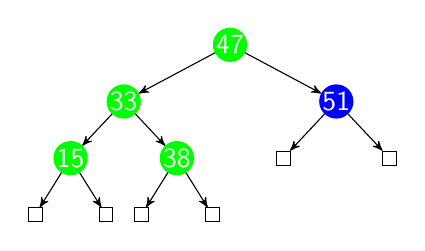
\begin{tikzpicture}[->,>=stealth',level/.style={sibling distance = 2.7cm/#1,level distance = 0.72cm}] 
				\node [arn_equi] {47}
	 				child{ node [arn_equi] {33} 
	        			child{ node [arn_equi] {15}
	    	         		child{ node [arn_null] {}
							}
							child{ node [arn_null] {}
							}       			 
	            		}                         
					  	child{ node [arn_equi] {38}
	    	         		child{ node [arn_null] {}
							}
							child{ node [arn_null] {}
							}  
						}
	            	}                            
	    		    child{ node [arn_new] {51}
	            		child{ node [arn_null] {}
						}
						child{ node [arn_null] {}
						}
	            	}			
			; 
			\end{tikzpicture}
		}
		\\
		\\
		\visible<3-4>{
			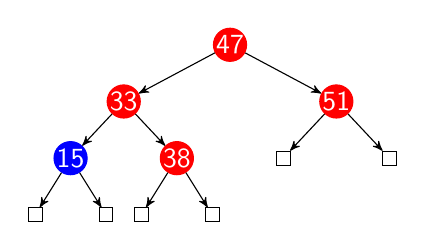
\begin{tikzpicture}[->,>=stealth',level/.style={sibling distance = 2.7cm/#1,level distance = 0.72cm}] 
				\node [arn_notequi] {47}
	 				child{ node [arn_notequi] {33} 
	        			child{ node [arn_new] {15}
	    	         		child{ node [arn_null] {}
							}
							child{ node [arn_null] {}
							}       			 
	            		}                         
					  	child{ node [arn_notequi] {38}
	    	         		child{ node [arn_null] {}
							}
							child{ node [arn_null] {}
							}  
						}
	            	}                            
	    		    child{ node [arn_notequi] {51}
	            		child{ node [arn_null] {}
						}
						child{ node [arn_null] {}
						}
	            	}			
			;  
			\end{tikzpicture}
		}
		&
		\visible<4>{
			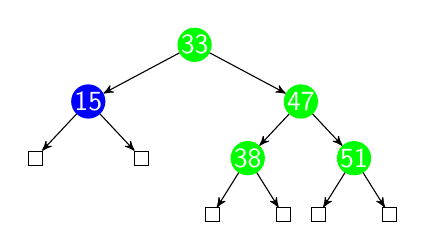
\begin{tikzpicture}[->,>=stealth',level/.style={sibling distance = 2.7cm/#1,level distance = 0.72cm}] 
				\node [arn_equi] {33}
	 				child{ node [arn_new] {15} 
	        			child{ node [arn_null] {}
						}
						child{ node [arn_null] {}
						}
	            	}                            
	    		    child{ node [arn_equi] {47}
	            		child{ node [arn_equi] {38} 
	            		    child{ node [arn_null] {}
							}
							child{ node [arn_null] {}
							}
	            		}
	            		child{ node [arn_equi] {51}
	            		    child{ node [arn_null] {}
							}
							child{ node [arn_null] {}
							}
	            		}
					}
			;
			\end{tikzpicture}
		}
		\\
		\multicolumn{2}{l}{
			\visible<3-4>{
				Diff de profondeur des ss-arbre de -2 et le FD une diff de -1.
			}
		}
		\\	
	\end{tabular}
\end{frame}

\begin{frame}{Equilibrage lors d'une insertion}
\framesubtitle{Rotation double droite gauche et gauche droite}
	\begin{tabular}{ccc}
	 	\multicolumn{2}{l}{
	 		\visible<1-4>{
	 			Diff de profondeur des ss-arbre de 2 et le FD une diff de -1.
	 		}
	 	}
	 	\\
	 	\visible<1-4>{
			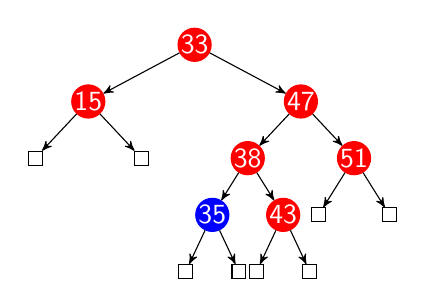
\begin{tikzpicture}[->,>=stealth',level/.style={sibling distance = 2.7cm/#1,level distance = 0.72cm}]
				\node [arn_notequi] {33}
	 				child{ node [arn_notequi] {15} 
	        			child{ node [arn_null] {}
						}
						child{ node [arn_null] {}
						}
	            	}                            
	    		    child{ node [arn_notequi] {47}
	            		child{ node [arn_notequi] {38}
	            			child{ node [arn_new] {35}
	            			    child{ node [arn_null] {}
								}
								child{ node [arn_null] {}
								}
							}
							child{ node [arn_notequi] {43}
							    child{ node [arn_null] {}
								}
								child{ node [arn_null] {}
								}
							}
	            		}
	            		child{ node [arn_notequi] {51}
	            		    child{ node [arn_null] {}
							}
							child{ node [arn_null] {}
							}
	            		}
					}
			; 
			\end{tikzpicture}
		}
		&
		\visible<2-4>{
			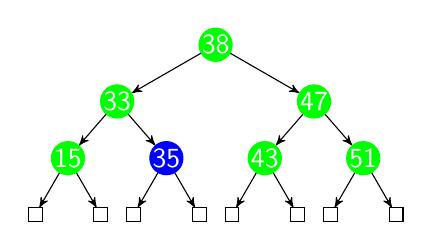
\begin{tikzpicture}[->,>=stealth',level/.style={sibling distance = 2.5cm/#1,level distance = 0.72cm}] 
				\node [arn_equi] {38}
	 				child{ node [arn_equi] {33} 
	        			child{ node [arn_equi] {15}
	    	         		child{ node [arn_null] {}
							}
							child{ node [arn_null] {}
							}       			 
	            		}                         
					  	child{ node [arn_new] {35}
	    	         		child{ node [arn_null] {}
							}
							child{ node [arn_null] {}
							}  
						}
	            	}                            
	    		    child{ node [arn_equi] {47}
	            		child{ node [arn_equi] {43}
	    	         		child{ node [arn_null] {}
							}
							child{ node [arn_null] {}
							}       			 
	            		}                         
					  	child{ node [arn_equi] {51}
	    	         		child{ node [arn_null] {}
							}
							child{ node [arn_null] {}
							}  
						}
	            	}			
			; 
			\end{tikzpicture}
		}
		\\
		\visible<3-4>{
			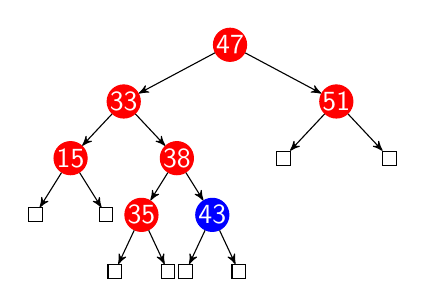
\begin{tikzpicture}[->,>=stealth',level/.style={sibling distance = 2.7cm/#1,level distance = 0.72cm}] 
				\node [arn_notequi] {47}
					child{ node [arn_notequi] {33}
	            		child{ node [arn_notequi] {15}
	            			child{ node [arn_null] {}
							}
							child{ node [arn_null] {}
							}
						}
			        	child{ node [arn_notequi] {38}
	            			child{ node [arn_notequi] {35}
	            			    child{ node [arn_null] {}
								}
								child{ node [arn_null] {}
								}
							}
							child{ node [arn_new] {43}
							    child{ node [arn_null] {}
								}
								child{ node [arn_null] {}
								}
							}
	            		}
					}
	 				child{ node [arn_notequi] {51} 
	        			child{ node [arn_null] {}
						}
						child{ node [arn_null] {}
						}
	            	}
			;  
			\end{tikzpicture} 
		}
		&
		\visible<4>{
			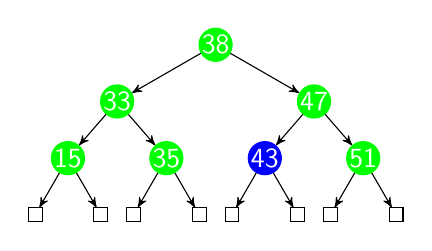
\begin{tikzpicture}[->,>=stealth',level/.style={sibling distance = 2.5cm/#1,level distance = 0.72cm}] 
				\node [arn_equi] {38}
	 				child{ node [arn_equi] {33} 
	        			child{ node [arn_equi] {15}
	    	         		child{ node [arn_null] {}
							}
							child{ node [arn_null] {}
							}       			 
	            		}                         
					  	child{ node [arn_equi] {35}
	    	         		child{ node [arn_null] {}
							}
							child{ node [arn_null] {}
							}  
						}
	            	}                            
	    		    child{ node [arn_equi] {47}
	            		child{ node [arn_new] {43}
	    	         		child{ node [arn_null] {}
							}
							child{ node [arn_null] {}
							}       			 
	            		}                         
					  	child{ node [arn_equi] {51}
	    	         		child{ node [arn_null] {}
							}
							child{ node [arn_null] {}
							}  
						}
	            	}			
			; 
			\end{tikzpicture}
		}
		\\
		 \multicolumn{2}{l}{
		 	\visible<4>{
		 		Diff de profondeur des ss-arbre de -2 et le FD une diff de 1.
		 	}
		 }
		 \\	
	\end{tabular}
\end{frame}

\section{Quoi}
\begin{frame}{Name}
	blblblblbl
\end{frame}


\end{document}

